\documentclass[14pt, a4paper]{extarticle}

\usepackage{my_GOST}
\usepackage{hyperref}
\usepackage{listings}
\usepackage{array}
\usepackage{caption}
\hypersetup{
	pdftex,
	colorlinks = true,
	linkcolor = black,
	filecolor = magenta,
	citecolor = green,      
	urlcolor = cyan,
}

% к таблице и листингу подпись сверху, перед каждым иллюстративным материалом анонсировать
% написатьт в квадратных скобках к рекурсии комментарием что это метод и понятно почему вызываем его снова
\definecolor{mylightgray}{RGB}{240,240,240}
\definecolor{mygreen}{rgb}{0,0.6,0}
\definecolor{mygray}{rgb}{0.5,0.5,0.5}
\definecolor{mymauve}{rgb}{0.58,0,0.82}

\lstset{
	backgroundcolor=\color{mylightgray},rulecolor=\color{red},  % choose the background color; you must add \usepackage{color} or \usepackage{xcolor}; should come as last argument
	basicstyle=\footnotesize\ttfamily,        % the size of the fonts that are used for the code
	breakatwhitespace=false,         % sets if automatic breaks should only happen at whitespace
	breaklines=true,                 % sets automatic line breaking
	captionpos=t,                    % sets the caption-position to bottom
	commentstyle=\color{mygreen},    % comment style
	extendedchars=false,              % lets you use non-ASCII characters; for 8-bits encodings only, does not work with UTF-8
	firstnumber=0,                % start line enumeration with line 1000
	frame=shadowbox,
	%rulesepcolor=\color{green},	                   % adds a frame around the code
	keepspaces=true,                 % keeps spaces in text, useful for keeping indentation of code (possibly needs columns=flexible)
	keywordstyle=\color{blue}\textbf,       % keyword style
	language=C++,                 % the language of the code
	morekeywords={*,...},            % if you want to add more keywords to the set
	numbers=left,                    % where to put the line-numbers; possible values are (none, left, right)
	numbersep=5pt,                   % how far the line-numbers are from the code
	numberstyle=\scriptsize\color{mygray}, % the style that is used for the line-numbers
	rulecolor=\color{black},         % if not set, the frame-color may be changed on line-breaks within not-black text (e.g. comments (green here))
	showspaces=false,                % show spaces everywhere adding particular underscores; it overrides 'showstringspaces'
	showstringspaces=false,          % underline spaces within strings only
	showtabs=false,                  % show tabs within strings adding particular underscores
	stepnumber=1,                    % the step between two line-numbers. If it's 1, each line will be numbered
	stringstyle=\color{mymauve},     % string literal style
	tabsize=4,	                   % sets default tabsize to 2 spaces
	title=\lstname                   % show the filename of files included with \lstinputlisting; also try caption instead of title
}
\usepackage{YATPR}

\usepackage[utf8]{inputenc}
\usepackage{amsmath}
\usepackage{float}

\begin{document}
\begin{titlepage}
	\newgeometry{pdftex, left=2cm, right=2cm, top=2.5cm, bottom=2.5cm}
	\fontsize{12pt}{12pt}\selectfont
	\noindent \begin{minipage}{0.15\textwidth}
		
\includegraphics[width=\linewidth]{pictures/b_logo.jpg}
	\end{minipage}
	\noindent\begin{minipage}{0.9\textwidth}\centering
		\textbf{Министерство науки и высшего образования Российской Федерации}\\
		\textbf{Федеральное государственное бюджетное образовательное учреждение высшего образования}\\
		\textbf{«Московский государственный технический университет имени Н.Э.~Баумана}\\
		\textbf{(национальный исследовательский университет)»}\\
		\textbf{(МГТУ им. Н.Э.~Баумана)}
	\end{minipage}
	
	\noindent\rule{18cm}{3pt}
	\newline\newline
	\noindent ФАКУЛЬТЕТ $\underline{\text{«Информатика и системы управления»}}$ \newline\newline
	\noindent КАФЕДРА $\underline{\text{«Программное обеспечение ЭВМ и информационные технологии»}}$\newline\newline\newline\newline\newline\newline\newline
	
	
	\begin{center}
		\Large\textbf{Отчет по лабораторной работе №2}\newline
	\end{center}
	
	\noindent\textbf{Название} $\underline{\text{~Марковские процессы~~~~~~~~~}}$\newline\newline\newline
	\noindent\textbf{Дисциплина} $\underline{\text{~Моделирование~~~~~~~~}}$\newline\newline
	\noindent\textbf{Студент} $\underline{\text{Егорова П. А.~~~~~~~~~~~~~~~~~~~~~~~~~~~~~~~~~~~~~~~~~}}$\newline\newline
	\noindent\textbf{Группа} $\underline{\text{ИУ7-74Б~~~~~~~~~~~~~~~~~~~~~~~~~~~~~~~~~~~~~~~~~~~~}}$\newline\newline
	\noindent\textbf{Оценка (баллы)} $\underline{\text{~~~~~~~~~~~~~~~~~~~~~~~~~~~~~~~~~~~~~~~~~~~~~~~~~}}$\newline\newline
	\noindent\textbf{Преподаватель}$\underline{\text{~Рудаков И. В.~~~~~~~~~~}}$\newline
	
	\begin{center}
		\vfill
		Москва~---~\the\year
		~г.
	\end{center}
 \restoregeometry
\end{titlepage}


\setcounter{page}{2}

\section{Задание}

Написать программу, которая генерирует алгоритмическим способом и получает табличным способом случайные последовательности одноразрядных, двухразрядных и трехразрядных целых чисел.

Разработать количественный критерий оценки случайности последовательности чисел. Для каждой полученной последовательности вычислить и вывести значение критерия.

Предусмотреть возможность ввода последовательности чисел и оценки их случайности с помощью критерия.


\section{Теоретические сведения}

\subsection{Способы получения случайных чисел}

На практике наиболее распространены 3 способа получения случайных чисел.

\textbf{Аппаратный способ}

При использовании аппаратного способа случайные числа вырабатываются специальной электронной приставкой (генератором случайных чисел). Реализация данного способа не требует дополнительных вычислений, необходима только одна операция -- обращение к вычислительному устройству. 

В качестве физического эффекта, лежащего в основе генерации случайных чисел, может использоваться, например, шум в электронных приборах.  Для генерации необходимы источник шума, ключевая схема, формирователь импульсов и пересчетная схема.

%Аппаратные генераторы случайных чисел – это устройства, использующие для создания случайных чисел замеры параметров некоторых физических процессов. Как правило, аппаратный генератор случайных чисел состоит из источника энтропии и устройства, преобразующего значения, полученные с источника энтропии, в нужный формат.


\textbf{Табличный способ}

Случайные числа берутся из заранее подготовленной таблицы, которая находится во внешней или оперативной памяти. Числа в таблице проверены на случайность и некоррелированы.



\textbf{Алгоритмический способ}

Алгоритмический способ основан на использовании специальных алгоритмов. К таким алгоритмам, например, относятся следующие:

\begin{itemize}
	\item алгоритм Фон-Неймана (метод серединных квадратов);
	\item метод перемешивания (сдвигов);
	\item вихрь Мерсенна;
	\item линейный конгруэнтный генератор;
\end{itemize}

Последний выбран для реализации в данной лабораторной работе. 

В этом методе каждое следующее число рассчитывается на основе предыдущего по формуле (\ref{formula1}).
\begin{equation}\label{formula1}
	R_{n + 1} = (a \cdot R_n + b)\;mod\;N,\, n \geq 1
\end{equation}
где a, b -- коэффициенты, N -- модуль.

Для качественного генератора требуется подобрать подходящие коэффициенты. Например, в таблице \ref{k} приведены некоторые из них.
\begin{table}[h]
	\begin{center}
		\caption{Примеры коэффициентов}
		\label{k}
		\begin{tabular}{| p{3cm} | p{3cm} | p{3cm}|}
			\hline
			\textbf{a} 			& \textbf{b} 	& \textbf{N} \\
			\hline
			106 				& 1283 			& 6075 \\ 
			\hline
			430 				& 2531  		& 11979 \\ 
			\hline
			84589 				& 15989 		& 217728 \\ 
			\hline
			1103515245 			& 12345 		& $2^{31}$ \\ 
			\hline
			... 				& ... 			& ... \\ 
			\hline
		\end{tabular}
	\end{center}
\end{table} 



\subsection{Критерий оценки случайности последовательности}

В рамках лабораторной работы в качестве статистической оценки используется критерий <<хи-квадрат>> ($\chi^2$-критерий).

Привлекая этот критерий можно оценить, удовлетворяет ли генератор требованию равномерного распределения или нет.

Используется статистика, представленная формулой (\ref{formula2}).
\begin{equation}\label{formula2}
	V = \frac{1}{n}\sum_{s=min}^{max} \left( \frac{Y_s^2}{p_s} \right) - n
\end{equation}
где n - длина последовательности, min/max - границы, в пределах которых находятся элементы последовательности, $Y_s$ - число повторений числа s, $p = \dfrac{1}{max - min}$.

Вычисляется квантиль хи-квадрат от вычисленного V. Если полученное значение будет меньше 0.1 или больше 0.9, то эти числа считаются недостаточно случайными. Если же нет, то последовательность принимается как случайная. 

\section{Результаты работы программы}

Интерфейс предполагает вывод первых 10 элементов из 1000 каждой последовательности (за исключением той, которую введёт пользователь, так как в этом случае длина фиксирована и равна 10). 

Результат работы программы приведен на рисунках \ref{pic:2}.. Можно заметить, что значения критерия в любом из столбцов находится в интервале от 0.1 до 0.9, что позволяет считать последовательности случайными.

\begin{figure}[ht!]
	\begin{center}
		{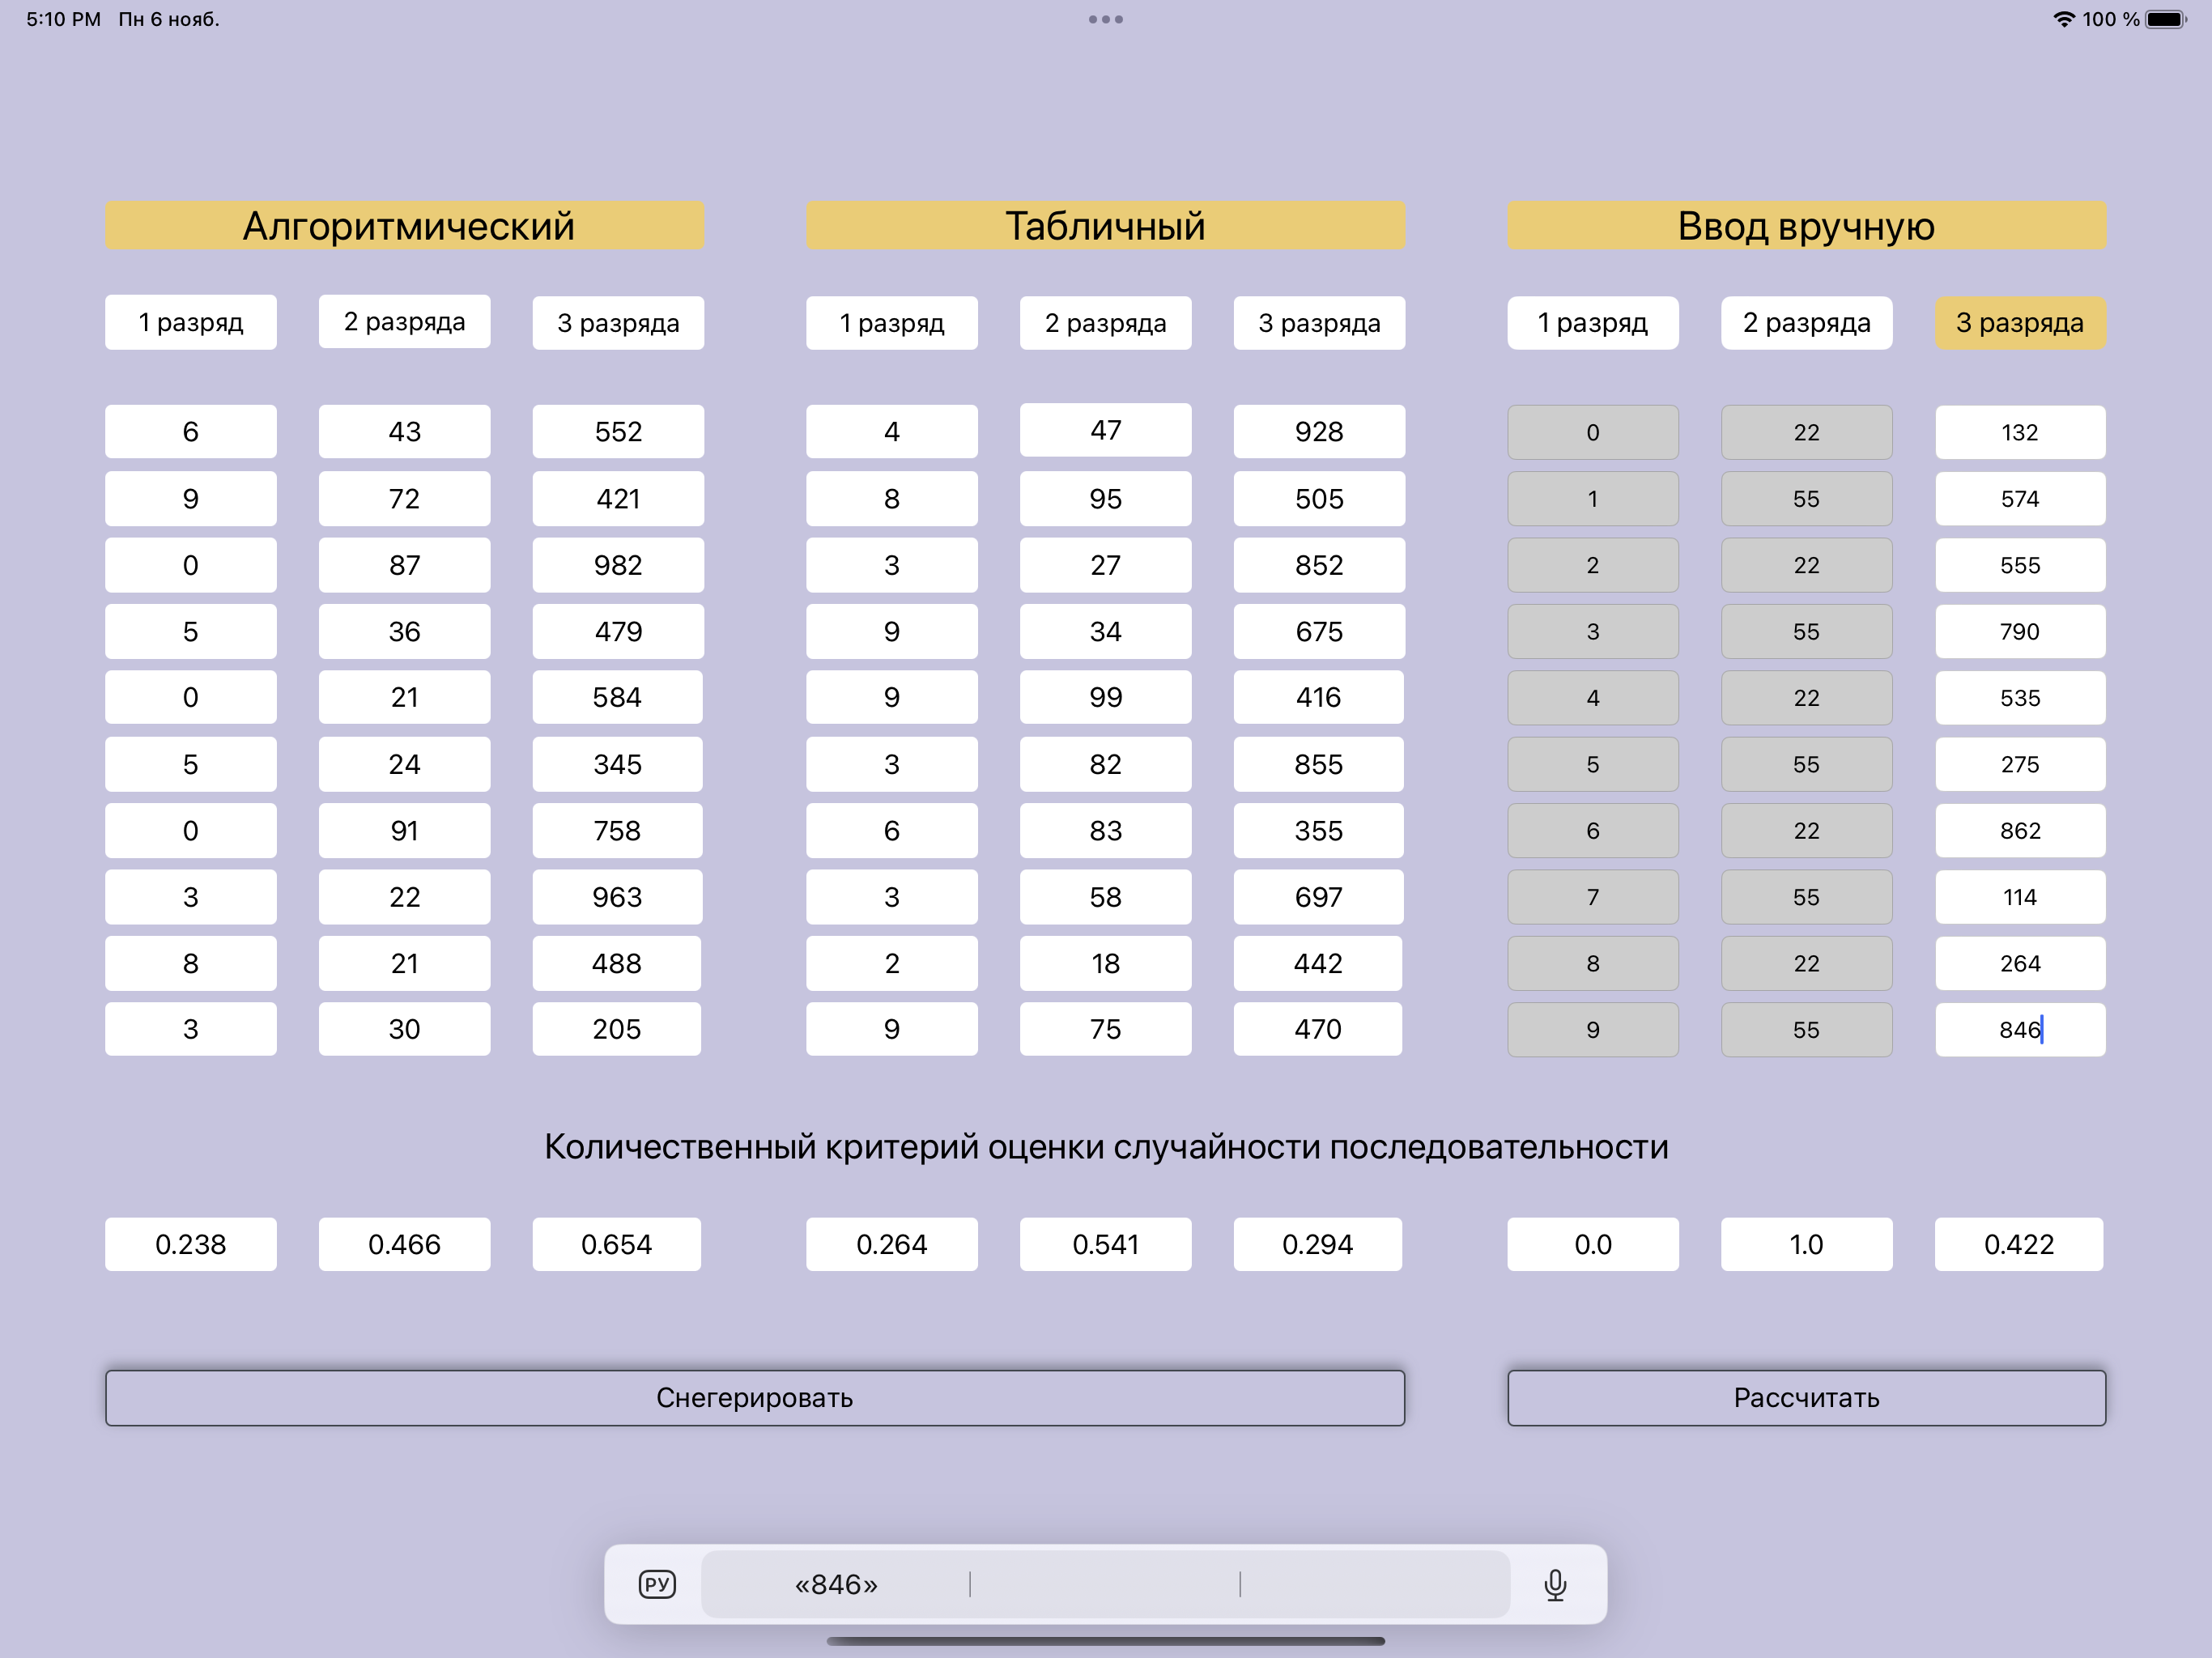
\includegraphics[scale=0.15]{pictures/res.png}
			\caption{Результаты работы}
			\label{pic:2}}
	\end{center}
\end{figure}

\newpage
\section{Код программы}
Код основной программы, которая инициирует генерацию последовательностей и рассчитывает критерии, приведен в листинге \ref{lst:list1} (используемый язык -- Swift).

\begin{lstlisting}[caption = {Код основной программы}, label=lst:list1]
class CongruentMethod {
    private let a: Int = 1103515245
    private let b: Int = 12345
    private let n: Int = Int(pow(Double(2), 31))
    private var r: Int
    
    init(seed: Int) {
        self.r = seed
    }
    
    func getNum(start: Int, end: Int) -> Int {
        r = (a * r + b) % n
        return r % (end - start) + start
    }
}

class AlgorithmMethod {
    let helpers = Helpers()
    
    func generateAlgorithmMethod(filename: String, start: Int, end: Int) {
        var arr = [String]()
        var nums = [Int]()
        let algorithmMethod = CongruentMethod(seed: Int.random(in: 0...100));

        for _ in 0..<1000 {
            let num = algorithmMethod.getNum(start: start, end: end)
            nums.append(num)
            arr.append("\(num)")
        }

        helpers.write_to_file(text: arr.joined(separator: "\n"), filename: filename)
    }
}
    
func generateTableMethod(filename: String, start: Int, end: Int) {
        let helpers = Helpers()
        var arr = Array(repeating: 0, count: 1000)
        let num = Int.random(in: 0...1000)
        var j = num

        var string = table1
        if start == 10 {
            string = table10
        }
        if start == 100 {
            string = table100
        }
        var nums = [Int]()
        let array = string.components(separatedBy: ",")
        for el in array { nums.append(Int(el)!) }

        for i in 0..<arr.count {
            arr[i] = nums[j]
            j = (j + 1) % nums.count
        }
        let elems = arr.map( {"\($0)"} )
        
        helpers.write_to_file(text: elems.joined(separator: "\n"), filename: filename)
    }
}

class Criteria {
    let helpers = Helpers()
    func getCriteria(filename: String, elMin: Int, elMax: Int) -> Double {
        let array = helpers.read_from_file(filename: filename).components(separatedBy: "\n")
        var nums = [Int]()
        for el in array { nums.append(Int(el)!) }
        var y = 0.0
        let p = 1.0 / Double(elMax - elMin)
        
        for i in elMin..<elMax {
            let count = nums.filter{ $0 == i }.count
            y += pow(Double(count), 2) / p
        }
        
        y = y / Double(nums.count) - Double(nums.count)
        
        do {
            let res = try cdfChiSquareDist(chi: y, degreesOfFreedom: Double(elMax - elMin - 1))
            return res
        } catch {
            return 0.0
        }
        
        return 0.0
    }
}
\end{lstlisting}

\end{document}